% -*- TeX:UK -*-
\chapter{Linear and linearising Regression}
\begin{refsection}

\abstract{In many cases, a dependent variable \AbsVec{y} can be described as linear function of an independent (predictor) variable \AbsVec{x}, using the criterion of minimal sum of squared residuals. Some important non-linear functions can be linearised by a suitable transformation of \AbsVec{x, y}; even if this results in biased estimates for the parameters. Non-parametric methods should be used for regression if the conditions of normality, uncorrelatedness and homoscedasticity of the error are violated.  }

The interface for the unit is
\begin{lstlisting}[caption=Interface]
  UNIT LinearRegression;

  INTERFACE

  USES math, MathFunc, Vector, Stat, Correlations;

  CONST RegressionError : BOOLEAN = FALSE;

  TYPE CurveTyp  = (Origin, Linear, Exponential, Power, Hyperbola, Inverse, Maximum,
                    Sigmoidal, ExpSigmoidal, ModPower, Hill);
       ResultTyp = RECORD
                     a, sa,                            // intercept
                     b, sb,                            // slope
                     m, sm,                            // exponent
                     r, t, P0 : double;                // TEST statistics
                   END;

  PROCEDURE Approximation(CONST x, y, weight : VectorTyp; ct : CurveTyp;
            VAR yCalc : VectorTyp; VAR Res : ResultTyp);
  // linear regression for least sum of squares

  PROCEDURE Transformation(CONST xOrig, yOrig : VectorTyp; VAR xTrans, yTrans : VectorTyp;
                           ct : CurveTyp; Schaetzwert : double);
  // transformation of x, y TO linearise

  PROCEDURE Retransform (CONST x, yTrans : Vectortyp; VAR TRes, Res : ResultTyp;
                         ct : CurveTyp; Schaetzwert : double;
                         VAR yCalc : VectorTyp);
  // re-transformation of linear results to curve

  PROCEDURE LinFit (Data : MatrixTyp;  mwt: BOOLEAN; VAR a, b, siga, sigb, chi2, q: real);
  { Robuste Daten-Modellierung nach Press et al.: Numerical Recepies in Pascal,
    Cambridge 1989, pp 590-8
    Anpassung von Daten an eine Ausgleichsgerade. Dabei wird jedoch die uebliche
    Annahme fallengelassen, alle Datenpunkte haetten die gleiche Standardabweichung.
    Eingabe: Data enthaelt die Daten, dabei stehen in jeder Zeile x, y und die
             Standardabweichung fuer y (falls letztere nicht zur Verfuegung
             stehen, muá mwt = false gesetzt werden).
    Ausgabe: a und b sind die Parameter des Modells, siga und sigb die Fehler-
             grenzen. chi2 ist ein Mass fuer die Guete des Modells, q die War-
             scheinlichkeit gegen dieses Modell. }

  PROCEDURE Deming (CONST x, y : VectorTyp; delta : double;
                    VAR xCalc, yCalc : VectorTyp; VAR Res : ResultTyp);
  // Deming regression for data with errors in x and y

  PROCEDURE TheilSenKendall (CONST x, y : VectorTyp; VAR yCalc : VectorTyp;
                             VAR Res : ResultTyp);
  // non-parametric regression

  PROCEDURE Eisenthal (CONST Substrate, Velocity : VectorTyp; VAR yCalc : VectorTyp;
                             VAR Res : ResultTyp);
  // Eisenthal & Cornish-Bowden 1974



  IMPLEMENTATION
\end{lstlisting}



\section{Linear regression}

For further information, consult \parencite{Noa-80,Spa-82,Wil-61,Abr-64}. Given a pair of vectors \AbsVec{x, y}, with \AbsVec{x} the independent (controlled, predictor) and \AbsVec{y} the dependent (predicted) variable, it is possible to calculate a line \(\hat{\AbsVec{y}} = f(\AbsVec{x}) = a + b \AbsVec{x} + \epsilon \) through these data pairs so that the sum of squared residuals \(\sum_{i=1}^{n}{(\AbsVec{y}_i - \hat{\AbsVec{y}}_i)^2} \) becomes minimal. Note that this is possible even when the data are not well represented by the model, in that case the fit will be poor, the squared residuals will be large and a plot of the residuals as function of \AbsVec{x} (or \(\hat{\AbsVec{y}} \)) will show a non-random pattern.

\begin{rules}
  Hence it is of utmost importance to \emph{always} plot both \(\AbsVec{y}_i \) and \(\hat{\AbsVec{y}}_i - \AbsVec{y}_i \) as function of \(\AbsVec{x}_i \) and to visually check these plots for unexpected patterns.
\end{rules}

The most common case of linear regression is data that are on a straight line, however, we speak of linear regression whenever the second and higher derivatives of the fitting function with respect to the parameters are all zero \parencite{Joh-10}.  Then the Gauss-Newton algorithm will require only a single iteration for any initial ‘‘guesses’’ of the fitting parameter values, which therefore can all be set to zero.

\subsection{Requirements for linear regression}

The data \AbsVec{x, y} should meet a couple of requirements:
\begin{itemize}
  \item{All error is in the \AbsVec{y}-vector, the \AbsVec{x}-vector is error-free. If both dependent and independent variables have errors, one can try a \Name{Deming} regression \parencite{Dem-43}.}
  \item{The error terms \(\epsilon \) should be \textbf{uncorrelated}, that is, knowledge of \(\epsilon_i \) should not allow the prediction of \(\epsilon_{i+1} \). For example, time series data are prone to correlations of error terms, because drift affects data the more similarly, the closer they are in time. A plot of \(\hat{\AbsVec{y}}_i - \AbsVec{y}_i \) as function of time can reveal this, perhaps followed by a runs test. Correlation of error may also occur if some data points have factors in common that the study doesn't test for. For example, in a study of height vs weight of persons, such correlations can arise if some test subjects were raised under the same environmental influences (say, in siblings), or if repeat measurements were made on the same subject. In effect, such correlations reduce the confidence intervals of parameters, making the data appear more precise than they actually are.}
  \item{The error should be \textbf{normally distributed}.}
  \item{\textbf{Homoscedasticity} of the data means that \(\AbsVec{y}_i - \hat{\AbsVec{y}}_i\) is independent of \AbsVec{x}. Depending on experimental design, especially for \AbsVec{y}-values spanning several orders of magnitude, \(\hat{\AbsVec{y}}_i - \AbsVec{y}_i \) may increase with \AbsVec{x}, so that the relative error stays constant. In a plot of residuals, one would see a funnel. Linear regression of such data by the least-squares criterion leads to biased parameters with underestimated standard deviations. A better approach would be a fit by minimal \(\chi^2 \), for example by the simplex algorithm (see chapter \ref{chap:Simplex} on page \pageref{chap:Simplex}). Alternatively, one can perform a weighted linear regression. }
  \item{The data should be free of \textbf{outliers}, that is, data points with extremely large residuals. Such data are obvious in a plot of the residuals. Even better is to plot the \emph{studentised residuals}, that is the residuals divided by their estimated standard error. Any data point with a studentised residual larger than \num{3} is suspect. If the outlier is the result of a measurement error, it should be removed. However, outliers may the result of an incomplete model (variables that affect the result, but were not accounted for). Robust (non-parametric) fitting methods, for example the \Name{Theil–Sen-Kendall}-estimator \parencite{The-50}, can be used if there are many outliers.  }
  \item{The distribution of data with respect to \AbsVec{x} should be reasonably even. Single data points with very extreme \AbsVec{x}-values may have a strong influence on the regression line, they have \textbf{high leverage}. Any problems with such data points will unduely affect the data fit. The leverage statistics for the \skalar{i}-th data point \(\AbsVec{h}_i = \frac{(\AbsVec{x}_i - \bar{\AbsVec{x}})^2}{\sum(\AbsVec{x} - \bar{\AbsVec{x}})^2} \) is a number \(0 \leq \AbsVec{h}_i \leq 1 \), and \(\bar{\AbsVec{h}} = \frac{p}{n} \). Thus any observation where \(\AbsVec{h}_i \gg \bar{\AbsVec{h}} \) is suspect. In multiple regression, \(\AbsVec{h} = \diag(\arr{H}) = \diag(\arr{X}(\arr{X}^T\arr{X})^{-1}\arr{X}^T) \) the diagonal of the hat-matrix.   }
\end{itemize}

\subsection{Algorithm}

\subsubsection{Parameters}

In matrix terms, the position of the minimum of the \acs{RSS} is given by \( \hat{\beta} = (\arr{X}^T \arr{X})^{-1} \arr{X}^T\AbsVec{y} \), its value by \( \mathrm{RSS}(\hat{\beta}) = \AbsVec{y}^T\AbsVec{y} - \hat{\beta}^T \arr{X}^T \arr{X} \hat{\beta} \) and the \acs{RSS} in the vicinity of the minimum by \( \mathrm{RSS}(\beta) = \mathrm{RSS}(\hat{\beta}) + (\beta - \hat{\beta})^T \arr{X}^T\arr{X}(\beta - \hat{\beta}) \) \parencite{Joh-10b}.

For a two-variable regression \( \hat{\AbsVec{y}}_i = a + b\AbsVec{x}_i \), the calculation is performed as follows:  With \(S_\AbsVec{x} = \sum_{i=1}^n{\AbsVec{x}_i} \), \(S_\AbsVec{y} = \sum_{i=1}^n{\AbsVec{y}_i} \), \(S_\AbsVec{xx} = \sum_{i=1}^n{(\AbsVec{x}_i^2)} \), \(S_\AbsVec{yy} = \sum_{i=1}^n{(\AbsVec{y}_i^2)} \), \(S_\AbsVec{xy} = \sum_{i=1}^n{(\AbsVec{x}_i\AbsVec{y}_i)} \), the estimated slope of the regression line \(b = \hat{\beta}_1 \) is
\begin{equation}
  b = \frac{n S_\AbsVec{xy} - S_\AbsVec{x}S_\AbsVec{y}}{n S_\AbsVec{xx} - S_\AbsVec{x}^2}
    = \frac{\mathrm{Cov}_{\AbsVec{x,y}}}{\mathrm{Var}_\AbsVec{x}}
\end{equation}
and the intercept \(a = \hat{\beta}_0 \)
\begin{equation}
  a = \bar{\AbsVec{y}} - b\bar{\AbsVec{x}}
\end{equation}
In other words, the regression line goes through the centroid of the data \((\bar{\AbsVec{x}}, \bar{\AbsVec{y}}) \) and is rotated until the sum of squared residuals is minimal.

A line can be forced through the origin, that is, \(a = 0 \). Then
\begin{equation}
  b = \frac{S_\AbsVec{xy}}{S_\AbsVec{xx}}
\end{equation}
Instead of (0,0), the line can go through any point (\skalar{h,k}):
\begin{equation}
  b = \frac{\overline{(\AbsVec{x} - h) (\AbsVec{y} - k)}}{\overline{(\AbsVec{x}-h)^2}}
    = \frac{\mathrm{Cov}_\AbsVec{x,y} + (\bar{\AbsVec{x}} - h) (\bar{\AbsVec{y}} - k)}{\mathrm{Var}_\AbsVec{x} + (\bar{\AbsVec{x}} - h)^2}
\end{equation}

\subsubsection{Correlation coefficient}

\Name{Pearson}'s product moment correlation between \AbsVec{x} and \AbsVec{y} is
\begin{equation}
 r = \frac{n S_\AbsVec{xy} - S_\AbsVec{x}S_\AbsVec{y}}{\sqrt{(n S_\AbsVec{xx} - S_\AbsVec{x}^2)(nS_\AbsVec{yy} - S_\AbsVec{y}^2)}}
\end{equation}
The square of \skalar{r} is the \textbf{coefficient of determination} \skalar{r^2}, the fraction of variance in the \AbsVec{y}-data that is explained by \AbsVec{x}. If the  \AbsVec{y}-data were predicted without knowledge of \AbsVec{x}, then one would use \(\bar{\AbsVec{y}} \) as best predictor, and the total error would be \(E_1 = \sum_{i=1}^n{(\AbsVec{y}_i - \bar{\AbsVec{y}})^2} \), the \textbf{\acf{TSS}}. If \AbsVec{x} is used for prediction, the new total error becomes \(E_2 = \sum_{i=1}^n{(\AbsVec{y}_i - \hat{\AbsVec{y}}_i)^2} \), the \textbf{\acf{RSS}}. Then \(r^2 = \frac{E_1 - E_2}{E_1} = 1 - \frac{E_2}{E_1} \), the \textbf{\acf{PRE}} from knowledge of \AbsVec{x} \parencite{Fre-65}. The \textbf{\acf{ESS}} \( = \sum_{i=1}^n{(\hat{\AbsVec{y}}_i - \bar{\AbsVec{y}})^2} = \mathrm{TSS} - \mathrm{RSS} \).

\begin{figure}
 \caption{\emph{Top}: Regression analysis for synthetic data (\num{100} data points, \(y = 1 + 2x \) with random noise added). The regression of \AbsVec{y} from \AbsVec{x} yields a different line from the regression of \AbsVec{x} from \AbsVec{y}. Both lines go through \((\bar{\AbsVec{x}}, \bar{\AbsVec{y}}) \), their angle \(\alpha \) is proportional to the correlation coefficient \skalar{r}. Note that the noise affects the estimate for the intercept much more than that for the slope. \emph{Bottom}: The residuals are randomly distributed around their average and show no discernible pattern. }
 \label{fig:CorReg}
 \centering
 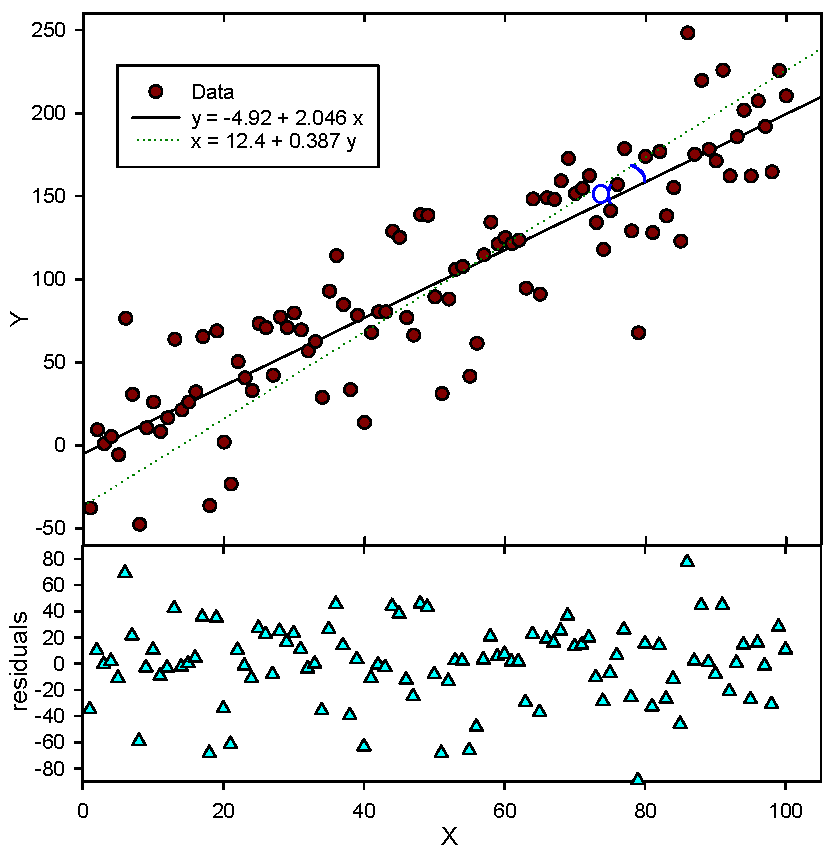
\includegraphics[width=0.75\textwidth]{Graphics/Correlation-Error}
\end{figure}

If one calculates the regression line between \AbsVec{x} and \AbsVec{y} with the parameters \(a_x, b_x \) and the regression line between \AbsVec{y} and \AbsVec{x} with the parameters \(a_y, b_y \) (see fig. \ref{fig:CorReg}), then these lines form an angle \(\alpha \) -- recall that both lines intersect at \((\bar{\AbsVec{x}}, \bar{\AbsVec{y}}) \). This angle is proportional to \skalar{r}, it is \ang{0} for \(r = 1 \) and \ang{90} for \(r = 0 \). The correlation coefficient is \(r = \sqrt{b_x b_y} \).

Yet another alternative interpretation of \skalar{r} is the slope of the regression line through the \skalar{z}-standardised data points. This line passes through the origin, because the arithmetic mean of \skalar{z}-standardised data is zero.

It is possible to test the regression for significance, that is, to test the 0-hypothesis \(H_0 : r = 0 \) against the alternative hypothesis \(H_1 : r \neq 0 \). For this, a \skalar{t}-value is calculated according to eqn. \ref{eqn:rt-sig}, then the degrees of freedom \(\nu = n - q \) is the number of measured values \skalar{n} minus the number of parameters used \skalar{q}.

In simple regression, \(R^2 = r^2 \), but in multiple regression, \(R^2 = \mathrm{Cor}(\AbsVec{y},\hat{\AbsVec{y}}) \neq r^2 \). The algorithm then maximises \(R^2 \).

It is sometimes necessary to decide between different models, with different number of parameters \(p \). Because
\begin{equation}
  R^2 = 1 - \frac{\sum{(\AbsVec{y}_i - \hat{\AbsVec{y}}_i)^2}}{\sum{(\AbsVec{y}_i - \bar{\AbsVec{y}})^2}}
\end{equation}
, \(R^2 \) will always increase with \(p \). This results from a reduction in training error, which may not correspond to a reduction in test error (overfitting). Thus, to compare models with different \(p \), we use the \textbf{adjusted \(R^2 \)}
\begin{equation}
  R^2_a = 1 - \frac{\sum{(\AbsVec{y}_i - \hat{\AbsVec{y}}_i)^2} / (n-p-1)}{\sum{(\AbsVec{y}_i - \bar{\AbsVec{y}})^2} / (n-1)}
\end{equation}
which may increase or decrease as additional parameters are added. Irrelevant parameters will decrease the sum of squared residuals only marginally, this is over-compensated by the increase of \(p \) in the denominator.
Other values used to identify the best number of parameters are
\begin{align}
  C_p          &= \frac{1}{n} \left(\sum_{i=1}^n{(\AbsVec{y}_i - \hat{\AbsVec{y}}_i)^2} + 2p\hat{\sigma}^2\right) \\
  \mathrm{AIC} &= \frac{1}{n\hat{\sigma}^2} \left(\sum_{i=1}^n{(\AbsVec{y}_i - \hat{\AbsVec{y}}_i)^2} + 2p\hat{\sigma}^2\right) \\
  \mathrm{BIC} &= \frac{1}{n} \left(\sum_{i=1}^n{(\AbsVec{y}_i - \hat{\AbsVec{y}}_i)^2} + \log(n)p\hat{\sigma}^2\right)
\end{align}
, which are closely related to each other. Whilst we are looking for a maximum of \(R^2 \), we look for the minimum of \(C_p \), \acs{BIC} and \acs{AIC}.

\subsubsection{Error estimates for the parameters \skalar{a, b}}

The variance of the residuals is
\begin{equation}
   s_\epsilon^2 = \frac{1}{n (n-2)} [n S_\AbsVec{yy} - S_\AbsVec{y}^2 - b^2 (n S_\AbsVec{xx} - S_\AbsVec{x}^2)]
\end{equation}
, the variance of \skalar{b}
\begin{equation}
  s_b^2 = \frac{n s_\epsilon^2}{n S_\AbsVec{xx} - S_\AbsVec{x}^2}
\end{equation}
and the variance of \skalar{a}
\begin{equation}
  s_a^2 = \frac{1}{n} s_b^2 S_\AbsVec{xx}
\end{equation}

The degrees of freedom is \(\nu = n - q \) with \skalar{q} the number of parameters  estimated, here 2. Given the 0.975-quantile of the \skalar{t}-distribution with \(\nu \) degrees of freedom \(t^*_\nu \), we can calculate the \SI{97.5}{\%} confidence intervals for the parameters to
\begin{equation}
  a \pm t^*_\nu \sqrt{s_a^2}\qquad  b \pm t^*_\nu \sqrt{s_b^2}
\end{equation}

\subsubsection{Tests for \(H_0: r=0 \), \(H_0: b=b_0 \) and \(H_0: a=a_0 \)  }

It is sometimes necessary to decide, whether there actually is a significant relationship between the dependent and independent variable, that is, we test \(H_0: r = 0 \) against \(H_1: r \neq 0 \). For this we can either do an \skalar{F}-test:
\begin{eqnarray}
  \nonumber
  F &=& \frac{r^2}{1-r^2} \\
  \nonumber
  \nu_1 &=& 1 \\
  \nu_2 &=& n-q
\end{eqnarray}
or a \skalar{t}-test:
\begin{eqnarray}
  \nonumber
  t &=& \sqrt{n-q \frac{r^2}{1-r^2}} \\
  \nu &=& n-q
\end{eqnarray}

Similarly, it may be interesting to test whether the \skalar{y}-intercept \skalar{a} is significantly different from any \skalar{a_0}. The most common application is \(a_0 = 0 \), \Foreign{i.e.}, are we looking at a line through the origin?
\begin{eqnarray}
 \nonumber
  t &=& \frac{|a-a_0|}{s_a} \\
  \nu &=& n-q
\end{eqnarray}

Lastly, one might wish to compare the slope \skalar{b} with some value \skalar{b_0}:
\begin{eqnarray}
 \nonumber
  t &=& \frac{|b-b_0|}{s_b} \\
  \nu &=& n-q
\end{eqnarray}
Again, the most common case is the test for \(b = 0 \).

\begin{lstlisting}[caption=Linear regression by RSS]
  PROCEDURE Approximation(CONST x, y, weight : VectorTyp; ct : CurveTyp;
            VAR yCalc : VectorTyp; VAR Res : ResultTyp);

  VAR Sx, Sy, Sw, Sxx, Syy, Sxy, SDxDy, SDx2, SDy2,xMean, yMean : double;
      c                                                         : CHAR;
      n                                                         : WORD;

    PROCEDURE DataSums;

    VAR
      i: INTEGER;
      DX, dy, xi, yi, wi : double;

    BEGIN
      Sx := 0;
      Sy := 0;
      Sw := 0;
      Sxy := 0;
      Sxx := 0;
      Syy := 0;
      SDxDy := 0;
      SDx2 := 0;
      SDy2 := 0;
      FOR i := 1 TO VectorLength(x) DO
        IF IsNaN(GetVectorElement(x, i)) OR IsNaN(GetVectorElement(y, i))
          THEN
          ELSE
            BEGIN
              xi := GetVectorElement(x, i);
              yi := GetVectorElement(y, i);
              wi := GetVectorElement(weight, i);
              Sx := Sx + xi * wi;
              Sy := Sy + yi * wi;
              Sw := Sw + wi;
              Sxy := Sxy + xi * yi * wi;
              Sxx := Sxx + xi * xi * wi;
              Syy := Syy + yi * yi * wi;
            END;
      xMean := Sx / Sw;
      yMean := Sy / Sw;
      FOR i := 1 TO VectorLength(x) DO
        IF IsNaN(GetVectorElement(x, i)) OR IsNaN(GetVectorElement(y, i))
          THEN
          ELSE
            BEGIN
              DX := GetVectorElement(x, i) - xMean;
              dy := GetVectorElement(y, i) - yMean;
              wi := GetVectorElement(Weight, i);
              SDxDy  := SDxDy + DX * dy * wi;
              SDx2 := SDx2  + DX * DX * wi;
              SDy2 := SDy2  + dy * dy * wi;
            END;
      SDxDy := SDxDy / Sw;
      SDx2  := SDx2  / Sw;
      SDy2  := SDy2  / Sw;
    END;


    PROCEDURE Parameters;

    VAR i: INTEGER;
        a1, a2, a3, a4 : double;

    BEGIN
      IF (ct = Origin)
        THEN
          BEGIN   // Line through origin
            Res.b := Sxy / Sxx;
            Res.a := 0;
          END
        ELSE
          BEGIN   // all others
            a1 := Sw * Sxy;
            a2 := Sx * Sy;
            a3 := Sw * Sxx;
            a4 := Sx * Sx;
            a4 := (a1-a2) / (a3-a4);
            Res.b := (Sw * Sxy - Sx * Sy) / (Sw * Sxx - Sx * Sx);
            Res.a := yMean - Res.b * xMean;
          END;
      FOR i := 1 TO VectorLength(x) DO
        IF IsNaN(GetVectorElement(x, i))
          THEN SetVectorElement(yCalc, i, NaN)
          ELSE SetVectorElement(yCalc, i, Res.a + Res.b * GetVectorElement(x, i));
    END;


    PROCEDURE ErrorEstimates;

    VAR i, f : INTEGER;
        Se : double;

    BEGIN
      CASE ct OF
        Origin            : f := Round(n - 1);    {degrees of freedom = data points - parameters}
        Linear..Maximum   : f := Round(n - 2);
        Sigmoidal..Hill   : f := Round(n - 3);
      END;
      WITH Res DO
        BEGIN
          se := 1/(Sw * f) * (Sw*Syy - Sy*Sy - Res.b*Res.b*(Sw*Sxx - Sx*Sx));
          sb := Sw*se / (Sw*Sxx - Sx*Sx);
          IF (ct = Origin)
            THEN sa := 0
            ELSE sa := (1/Sw) * sb *Sxx;
          se := Sqrt(se);
          sa := Sqrt(Res.sa);
          sb := Sqrt(Res.sb);
          r := SDxDy / Sqrt(SDx2 * SDy2);
          IF (r < 1)  // prevent division by 0
            THEN
              BEGIN
                t := r * Sqrt(f/(1-r*r));
                P0 := Integral_t(t, f);
              END
            ELSE
              BEGIN
                t := NaN;
                P0 := 0;
              END;
        END;
    END;

  BEGIN
    IF VectorLength(x) <> VectorLength(y)
      THEN
        BEGIN
          c := WriteErrorMessage('Linear regression: unequal length of dependent and independent data vector');
          RegressionError := TRUE;
          EXIT;
        END;
    n := VectorLength(x);
    CreateVector(yCalc, VectorLength(x), 0.0);
    DataSums;
    Parameters;
    ErrorEstimates;
  END;
\end{lstlisting}

\section{Weighted regression}

Sometimes, the data points have uneven standard deviation, that is, they are not homoscedastic. In that case, we can weight the data points with the reciprocal of their standard deviation. Then
\begin{eqnarray}
  \nonumber
  \bar{\AbsVec{x}} &=& \frac{\sum(\AbsVec{w}_i\AbsVec{x}_i)}{\sum(\AbsVec{w}_i)} \\
  \nonumber
  \bar{\AbsVec{y}} &=& \frac{\sum(\AbsVec{w}_i\AbsVec{y}_i)}{\sum(\AbsVec{w}_i)} \\
  \nonumber
  b &=& \frac{\sum(\AbsVec{w}_i (\AbsVec{x}_i-\bar{\AbsVec{x}}) (\AbsVec{y}_i-\bar{\AbsVec{y}}))}{\sum(\AbsVec{w}_i (\AbsVec{x}_i-\bar{\AbsVec{x}})^2)} = \frac{\sum(\AbsVec{w}_i\AbsVec{x}_i\AbsVec{y}_i) - \sum(\AbsVec{w}_i\AbsVec{x}_i) \sum(\AbsVec{w}_i\AbsVec{y}_i)/\sum(\AbsVec{w}_i)}{\sum(\AbsVec{w}_i\AbsVec{x}_i^2) - (\sum(\AbsVec{w}_i\AbsVec{x}_i))^2 / \sum\AbsVec{w}_i} \\
  \nonumber
  a &=& \bar{\AbsVec{y}} - b \bar{\AbsVec{x}} \\
  \nonumber
  s_y^2 &=& \frac{\sum(\AbsVec{w}_i (\AbsVec{y}_i - \hat{\AbsVec{y}}_i)}{n-q} = \frac{\sum(\AbsVec{w}_i\AbsVec{y}_i^2) - \bar{y}\sum(\AbsVec{w}_i\AbsVec{y}_i) - b \sum(\AbsVec{w}_i (\AbsVec{x}_i - \bar{\AbsVec{x}}) (\AbsVec{y}_i - \bar{\AbsVec{y}}))}{n-q} \\
  \nonumber
  s_b^2 &=& \frac{s_y^2}{\sum(\AbsVec{w}_i (\AbsVec{x}_i - \bar{\AbsVec{x}})^2)} \\
  s_a^2 &=& s_y^2 \left[\frac{1}{\sum(\AbsVec{w}_i)} + \frac{\bar{\AbsVec{x}}^2}{\sum(\AbsVec{w}_i (\AbsVec{x} - \bar{\AbsVec{x}})^2)} \right]
\end{eqnarray}
In case the line is supposed to go through the origin, \(a = 0 \), replace all \(\AbsVec{x}_i \) with \((\AbsVec{x}_i - \bar{\AbsVec{x}}) \) and \(s_y^2 = \frac{\sum(\AbsVec{w}_i\AbsVec{y}_1^2) - b \sum(\AbsVec{w}_i (\AbsVec{x}_i - \bar{\AbsVec{x}}) (\AbsVec{y}_i - \bar{\AbsVec{y}}))}{n-1} \).

\section{Robust linear regression}

Sometimes we want to calculate a regression line when the data are not homoscedastic. The following procedure \parencite[pp. 590-8]{Pre-89} allows us to do this. The data have three columns: \skalar{x, y} and the standard deviation of \skalar{y}. If the latter is not available, the variable \texttt{mwt} must be set to \texttt{FALSE}.

\begin{lstlisting}[caption=Robust linear regression]
PROCEDURE LinFit (Data : MatrixTyp;  mwt: BOOLEAN; VAR a, b, siga, sigb, chi2, q: real);

VAR i, nData            : INTEGER;
    wt, t, sy, sxoss,
    sx, st2, ss, sigdat : float;

BEGIN
   sx := 0.0;
   sy := 0.0;
   st2 := 0.0;
   b := 0.0;
   nData := MatrixRows(Data);
   IF mwt
     THEN
       BEGIN
         ss := 0.0;
         FOR i := 1 TO ndata DO
           BEGIN
             wt := 1.0 / Sqr(GetMatrixElement(Data, i, 3));
             ss := ss + wt;
             sx := sx + GetMatrixElement(Data, i, 1) * wt;
             sy := sy + GetMatrixElement(Data, i, 2) * wt
           END
      END
     ELSE
       BEGIN
         FOR i := 1 TO ndata DO
            BEGIN
                sx := sx + GetMatrixElement(Data, i, 1);
                sy := sy + GetMatrixElement(Data, i, 2);
            END;
         ss := ndata
       END;
   sxoss := sx/ss;
   IF mwt
     THEN
       BEGIN
         FOR i := 1 TO ndata DO
           BEGIN
             t := (GetMatrixElement(Data, i, 1) -sxoss) / GetMatrixElement(Data, i, 3);
             st2 := st2+t*t;
             b := b + t * GetMatrixElement(Data, i, 2) / GetMatrixElement(Data, i, 3);
           END
       END
     ELSE
       BEGIN
         FOR i := 1 TO ndata DO
           BEGIN
             t := GetMatrixElement(Data, i, 1) - sxoss;
             st2 := st2 + t * t;
             b := b + t * GetMatrixElement(Data, i, 2);
           END
       END;
   b := b / st2;
   a := (sy - sx * b) / ss;
   siga := Sqrt((1.0 + sx * sx / (ss * st2)) / ss);
   sigb := Sqrt(1.0 / st2);
   chi2 := 0.0;
   IF NOT mwt
     THEN
       BEGIN
         FOR i := 1 TO ndata DO
           chi2 := chi2 + Sqr(GetMatrixElement(Data, i, 2) - a - b * GetMatrixElement(Data, i, 1));
         q := 1.0;
         sigdat := Sqrt(chi2 / (ndata - 2));
         siga := siga * sigdat;
         sigb := sigb * sigdat;
       END
     ELSE
       BEGIN
         FOR i := 1 TO ndata DO
           chi2 := chi2 + Sqr((GetMatrixElement(Data, i, 2) - a - b *
                   GetMatrixElement(Data, i, 1)) / GetMatrixElement(Data, i, 3));
         q := IntegralChi(chi2, ndata-2);
       END;
END;
\end{lstlisting}


\section{Linearising regression}

\begin{figure}
 \caption{Linearising regression. \emph{Left, red}: Artificial data following a hyperbolic curve \(\hat{\AbsVec{y}} = \frac{1.0 \times \AbsVec{x}}{1.0 + \AbsVec{x}} \) with added noise. The residuals are random, without discernible pattern. \emph{Right}: The same data, linearised by taking reciprocals of both \AbsVec{x} and \AbsVec{y}. The residuals increase with \(1/\AbsVec{x} \) (\emph{pink shade}), they are no longer homoscedastic. As a result, the residuals of the re-transformed data increase with \AbsVec{x} (\emph{lower left, green triangles} and \emph{line}). The resulting hyperbolic curve (\emph{upper left, green line}) poorly represents the data at high \AbsVec{x}.}
 \label{fig:LinReg}
 \centering
 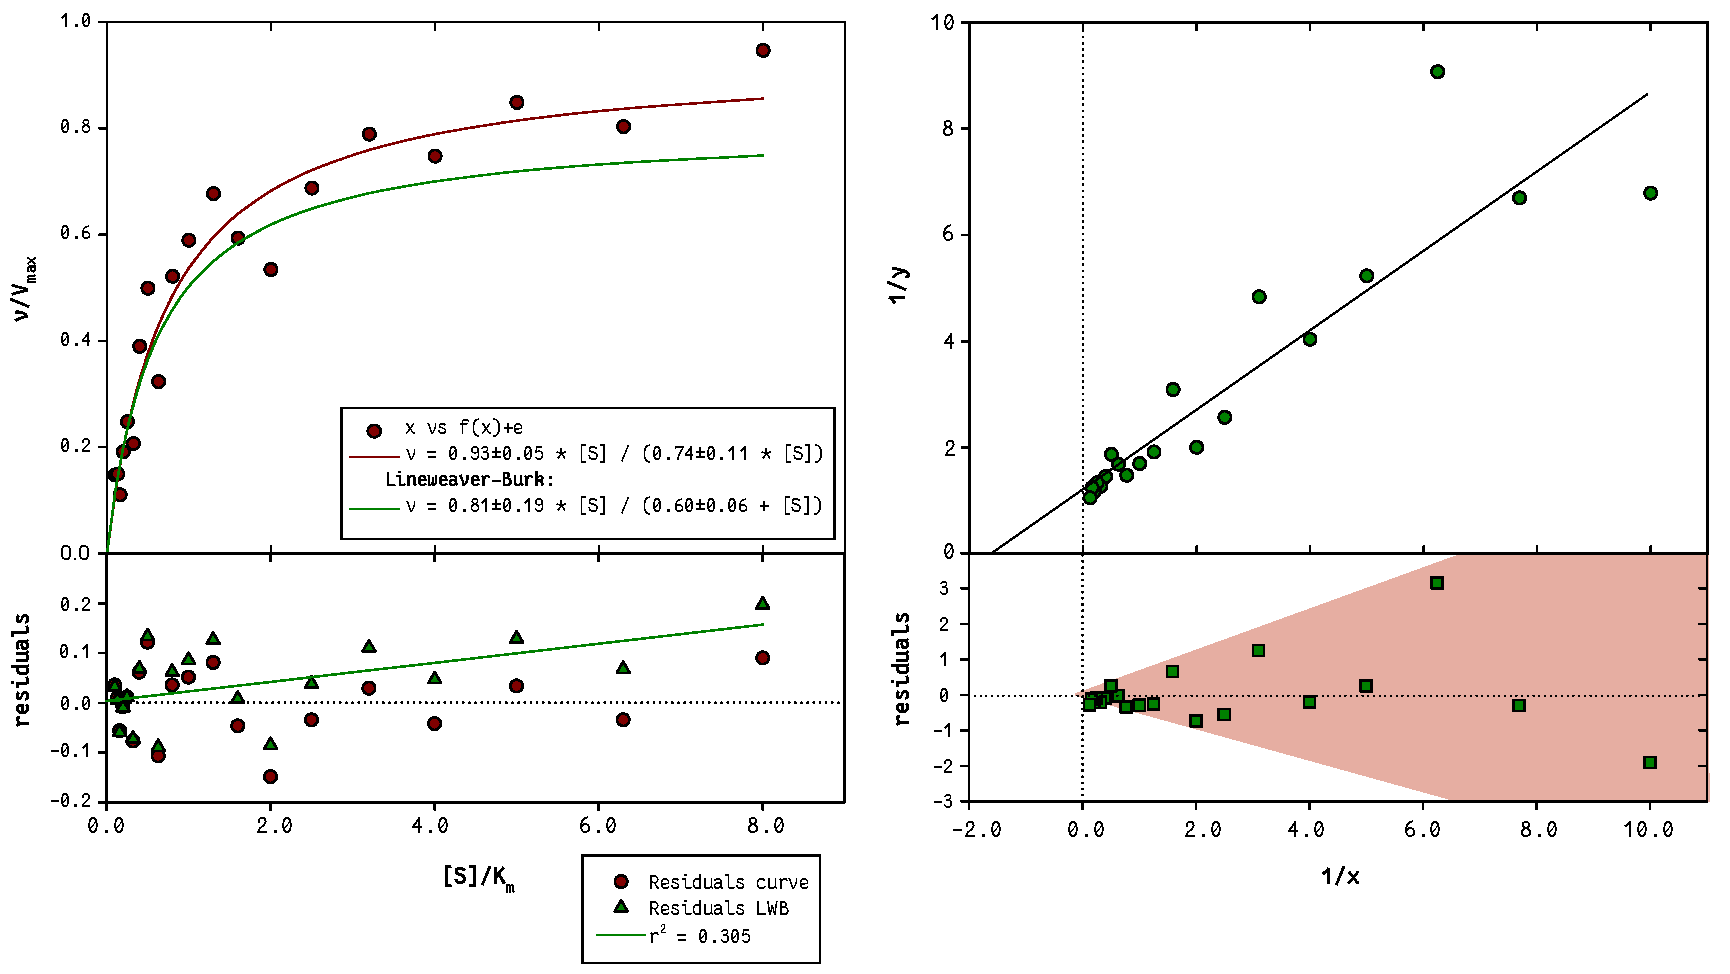
\includegraphics[width=\textwidth]{Graphics/LinearisingRegression}
\end{figure}

\begin{figure}
 \caption{\emph{Top}: Distribution of \num{200} normally distributed random figures. \emph{Bottom}: The distribution of the same data after taking reciprocals. The reciprocal of a \Name{Gauss}ian is not \Name{Gauss}ian!}
 \label{fig:RecGau}
 \centering
 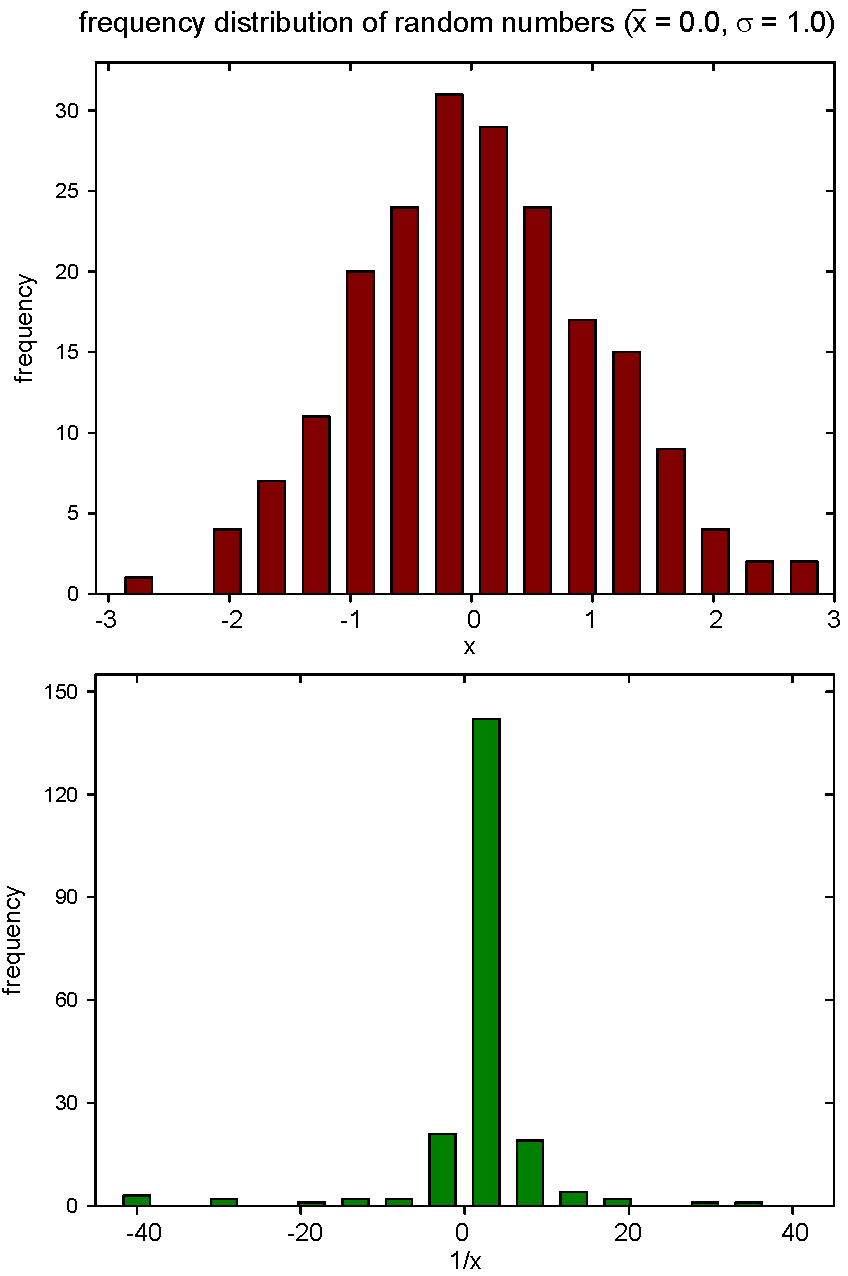
\includegraphics[width=0.75\textwidth]{Graphics/Reciprocal-Gaussian}
\end{figure}

Before computers became generally available, which allowed curve fitting by iterative methods, regression to suitably transformed data was generally used for curve fitting. The biggest disadvantage of these methods was that any method that transforms \AbsVec{y}, implicitly also transforms its error distribution. As a consequence, the requirements of homoscedasticity (see fig. \ref{fig:LinReg}) and of normality (see fig. \ref{fig:RecGau}) are violated, leading to biased estimates of parameters and, more importantly, their standard deviation. Note that this applies only to transformations of the dependent variable, as the independent variable is assumed to be error free its error distribution cannot be affected by transformation. Plots of transformed data still have a place in science for presentation purposes, as the human eye is very sensitive to deviations from a straight line. However, regression analysis of such data is largely obsolete.

Iterative regression methods require starting estimates of the parameters that should be reasonably close to the final value, firstly to reduce the number of iterations required and hence computer time. Secondly, iterative methods can become trapped in local minima of the error function, and then deliver suboptimal results. In my experience, the \Name{Levenberg-Marquardt}-algorithm \parencite{Lev-44,Mar-63} is more sensitive to this than \Name{Nelder-Mead}'s simplex algorithm \parencite{Nel-65,Cac-84,Kim-97}. Although the parameter estimates from linearising regression are biased, they are certainly good enough as starting values for iterative methods.

\begin{sidewaystable}
 \caption{Equations used in linearising regression. For the top equations, regression can happen directly, the bottom equations require an estimated parameter, either the \(y_\mathrm{max} \) or \(y_{x=0} \), respectively. The weights can be used to counteract the effect of the transformation on the error of the \AbsVec{y}-value.}
 \label{tab:linearise}
 \centering
 \begin{tabular}{rllllllll}
 \toprule
 No & Name                & Equation             & x-transform         & y-transform                                 & weight                                                    & \(a = \)            & \(b = \)       & \(m = \)  \\
 \midrule
  0 & Line through origin & \(y=b*x \)              & \(x^* = x \)            & \(y^* = y \)                                  & 1                                                         & \(a^* \)            & \(b^* \)       &        \\
  1 & linear              & \(y=a + b*x \)          & \(x^* = x \)            & \(y^* = y \)                                  & 1                                                         & \(a^* \)            & \(b^* \)       &        \\
  2 & exponential         & \(y=a*e^{m*x} \)        & \(x^* = x \)            & \(y^* = \ln(y) \)                             & \(y^2 \)                                                     & \(\exp(a^*) \)      &             & \(b^* \)  \\
  3 & power               & \(y=a*x^m \)            & \(x^* = \ln(x) \)       & \(y^* = \ln(y) \)                             & \(y^2 \)                                                     & \(\exp(a^*) \)      &             & \(b^* \)  \\
  4 & hyperbolic          & \(y=(a*x)/(b+x) \)      & \(x^* = 1/x \)          & \(y^* = 1/y \)                                & \(y^4 \)                                                     & \(1/a^* \)          & \(b^* a \)     &        \\
  5 & modif.invers        & \(y=a/(b+x) \)          & \(x^* = x \)            & \(y^* = 1/y \)                                & \(y^4 \)                                                     & \(1/b^* \)          & \(a^* a \)     &        \\
  6 & maximum             & \(y=a*x*e^{m*x} \)      & \(x^* = x \)            & \(y^* = \ln(x/y) \)                           & \((x * y)^2 / (y - x)^2 \)                                   & \(\exp(-a^*) \)     &             & \(-b^* \) \\
 \midrule
  7 & sigmoidal           & \(y=a/(1+b*x^m) \)      & \(x^* = \ln(x) \)       & \(y^* = \ln(y_\mathrm{max}/y - 1) \)          & \((y_\mathrm{max}/y - 1)^2 / (y_\mathrm{max} / y^2)^2 \)     & \(y_\mathrm{max} \) & \(\exp(a^*) \) & \(b^* \)  \\
  8 & exp.sigmoidal       & \(y=a/(1+b*exp(m*x)) \) & \(x^* = x \)            & \(y^* = \ln(y_\mathrm{max}/y - 1) \)          & \((y_\mathrm{max}/y - 1)^2 / (y_\mathrm{max} / y^2)^2 \)     & \(y_\mathrm{max} \) & \(\exp(a^*) \) & \(b^* \)  \\
  9 & mod. power          & \(y=a*x^m +b \)         & \(x^* = \ln(x) \)       & \(y^* = \ln(y - y_{x=0}) \)                   & \((y - y_{x=0})^2 \)                                         & \(y_{x=0} \)        & \(\exp(a^*) \) & \(b^* \)  \\
 10 & Hill                & \(y=a*x^m / (b+x^m) \)  & \(x^* = \log_{10}(x) \) & \(y^* = \log_{10}(y/ (y_\mathrm{max} - y)) \) & \(y^2 / \log_{10}(\mathrm{e} * (y_\mathrm{max}^2 - y))^2 \)  & \(y_\mathrm{max} \) & \(10^{-a} \)   & \(b^* \)  \\
 \bottomrule
 \end{tabular}
\end{sidewaystable}

\begin{lstlisting}[caption=Linearisation of curved data]
  PROCEDURE Transformation(CONST xOrig, yOrig : VectorTyp; VAR xTrans, yTrans : VectorTyp;
                           ct : CurveTyp; Schaetzwert : double);
  // transformation OF x, y TO linearise

  VAR i, n : INTEGER;

  BEGIN
      n := VectorLength(xOrig);
      CreateVector(xTrans, n, 0.0);
      CreateVector(yTrans, n, 0.0);
      FOR i := 1 TO n DO
        IF IsNaN(GetVectorelement(xOrig, i))
          THEN
            SetVectorElement(xTrans, i, NaN)
          ELSE
            CASE ct OF                        {Transformation of x-values}
              Origin, Linear, Exponential, Inverse, Maximum, ExpSigmoidal :
                 SetVectorElement(xTrans, i, GetVectorElement(xOrig, i));
              Power, Sigmoidal, ModPower :
                 SetVectorElement(xTrans, i, Ln(GetVectorElement(xOrig, i)));
              Hyperbola :
                 SetVectorElement(xTrans, i, 1 / GetVectorElement(xOrig, i));
              Hill :
                 SetVectorElement(xTrans, i, log(GetVectorElement(xOrig, i), 10));
            END;
      FOR i := 1 TO n DO
        IF IsNaN(GetVectorelement(yOrig, i))
          THEN
            SetVectorElement(yTrans, i, NaN)
          ELSE
            CASE ct OF                 {Transformation of y-values}
              Origin, Linear          :  SetVectorElement(yTrans, i, GetVectorElement(yOrig, i));
              Exponential, Power      :  SetVectorElement(yTrans, i, Ln(GetVectorElement(yOrig, i)));
              Hyperbola, Inverse      :  SetVectorElement(yTrans, i, 1 / GetVectorElement(yOrig, i));
              Maximum                 :  IF IsNaN(GetVectorelement(xOrig, i))
                                           THEN SetVectorElement(yTrans, i, NaN)
                                           ELSE SetVectorElement(yTrans, i, Ln(GetVectorElement(xOrig, i) / GetVectorElement(yOrig, i)));
              Sigmoidal, ExpSigmoidal :  SetVectorElement(yTrans, i, Ln(Schaetzwert / GetVectorElement(yOrig, i) - 1));
              ModPower                :  SetVectorElement(yTrans, i, Ln(GetVectorElement(yOrig, i) - Schaetzwert));
              Hill                    :  SetVectorElement(yTrans, i, log(GetVectorElement(yOrig, i) / (Schaetzwert - GetVectorElement(yOrig, i)), 10));
            END;
  END;


  PROCEDURE Retransform (CONST x, yTrans : Vectortyp; VAR TRes, Res : ResultTyp;
                         ct : CurveTyp; Schaetzwert : double;
                         VAR yCalc : VectorTyp);

  VAR i, n : WORD;

  BEGIN
    n := VectorLength(x);
    CreateVector(yCalc, n, 0.0);
    CASE ct OF
      Origin, Linear : BEGIN
                         CopyVector(yTrans, yCalc);
                         Res := TRes;
                         Res.m := 0;
                         Res.sm := 0;
                       END;
      Exponential    : BEGIN
                         Res.a  := Exp(TRes.a);
                         Res.sa := TRes.sa/Tres.a * Res.a;
                         Res.b  := 0;
                         Res.sb := 0;
                         Res.m  := TRes.b;
                         Res.sm := TRes.sb;
                         CreateVector(yCalc, VectorLength(yTrans), 0.0);
                         FOR i := 1 TO n DO
                           BEGIN
                             IF IsNaN(GetVectorElement(yTrans, i))
                               THEN SetVectorElement(yCalc, i, NaN)
                               ELSE SetVectorElement(yCalc, i, Res.a *
                                      Exp(Res.m * GetVectorElement(x, i)));
                           END;
                       END;
      Power          : BEGIN
                         Res.a  := Exp(TRes.a);
                         Res.sa := TRes.sa/Tres.a * Res.a;
                         Res.b  := 0;
                         Res.sb := 0;
                         Res.m  := TRes.b;
                         Res.sm := TRes.sb;
                         CreateVector(yCalc, VectorLength(yTrans), 0.0);
                         FOR i := 1 TO n DO
                           BEGIN
                             IF IsNaN(GetVectorElement(yTrans, i))
                               THEN SetVectorElement(yCalc, i, NaN)
                               ELSE SetVectorElement(yCalc, i, Res.a *
                                      Pot(GetVectorElement(x, i), Res.m)) ;
                           END;
                       END;
      Hyperbola      : BEGIN
                         Res.a  := 1/TRes.a;
                         Res.sa := TRes.sa/Tres.a * Res.a;
                         Res.b  := Tres.b * Res.a;
                         Res.sb := TRes.sb/Tres.b * Res.b;
                         Res.m  := 0;
                         Res.sm := 0;
                         CreateVector(yCalc, VectorLength(yTrans), 0.0);
                         FOR i := 1 TO n DO
                           BEGIN
                             IF IsNaN(GetVectorElement(yTrans, i))
                               THEN SetVectorElement(yCalc, i, NaN)
                               ELSE SetVectorElement(yCalc, i, Res.a * GetVectorElement(x, i)
                                       / (Res.b + GetVectorElement(x, i)));
                           END;
                       END;
      Inverse        : BEGIN
                         Res.a  := 1/TRes.b;
                         Res.sa := TRes.sb/Tres.b * Res.a;
                         Res.b  := Tres.a * Res.a;
                         Res.sb := TRes.sa/Tres.a * Res.b;
                         Res.m  := 0;
                         Res.sm := 0;
                         CreateVector(yCalc, VectorLength(yTrans), 0.0);
                         FOR i := 1 TO n DO
                           BEGIN
                             IF IsNaN(GetVectorElement(yTrans, i))
                               THEN SetVectorElement(yCalc, i, NaN)
                               ELSE SetVectorElement(yCalc, i, Res.a /
                                      (Res.b + GetVectorElement(x, i)));
                           END;
                       END;
      Maximum        : BEGIN
                         Res.a  := Exp(-TRes.a);
                         Res.sa := Abs(TRes.sa/Tres.a * Res.a);
                         Res.b  := 0;
                         Res.sb := 0;
                         Res.m  := -TRes.b;
                         Res.sm := Abs(TRes.sb/Tres.b * Res.m);
                         CreateVector(yCalc, VectorLength(yTrans), 0.0);
                         FOR i := 1 TO n DO
                           BEGIN
                             IF IsNaN(GetVectorElement(yTrans, i))
                               THEN SetVectorElement(yCalc, i, NaN)
                               ELSE SetVectorElement(yCalc, i, Res.a * GetVectorElement(x, i)
                                       * Exp(Res.m * GetVectorElement(x, i)));
                           END;
                       END;
      Sigmoidal      : BEGIN
                         Res.a  := Schaetzwert;
                         Res.sa := NaN;
                         Res.b  := Exp(TRes.a);
                         Res.sb := TRes.sa/Tres.a * Res.a;
                         Res.m  := TRes.b;
                         Res.sm := TRes.sb/Tres.b * Res.m;
                         CreateVector(yCalc, VectorLength(yTrans), 0.0);
                         FOR i := 1 TO n DO
                           BEGIN
                             IF IsNaN(GetVectorElement(yTrans, i))
                               THEN SetVectorElement(yCalc, i, NaN)
                               ELSE SetVectorElement(yCalc, i, Res.a /
                                      (1 + Res.b * Pot(GetVectorElement(x, i), Res.m)));
                           END;
                       END;
      ExpSigmoidal   : BEGIN
                         Res.a  := Schaetzwert;
                         Res.sa := NaN;
                         Res.b  := Exp(TRes.a);
                         Res.sb := TRes.sa/Tres.a * Res.a;
                         Res.m  := TRes.b;
                         Res.sm := TRes.sb/Tres.b * Res.m;
                         CreateVector(yCalc, VectorLength(yTrans), 0.0);
                         FOR i := 1 TO n DO
                           BEGIN
                             IF IsNaN(GetVectorElement(yTrans, i))
                               THEN SetVectorElement(yCalc, i, NaN)
                               ELSE SetVectorElement(yCalc, i, Res.a /
                                      (1 + Res.b * Exp(GetVectorElement(x, i) * Res.m)));
                           END;
                       END;
      ModPower       : BEGIN
                         Res.a  := Schaetzwert;
                         Res.sa := NaN;
                         Res.b  := Exp(TRes.a);
                         Res.sb := TRes.sa/Tres.a * Res.a;
                         Res.m  := TRes.b;
                         Res.sm := TRes.sb/Tres.b * Res.m;
                         CreateVector(yCalc, VectorLength(yTrans), 0.0);
                         FOR i := 1 TO n DO
                           BEGIN
                             IF IsNaN(GetVectorElement(yTrans, i))
                               THEN SetVectorElement(yCalc, i, NaN)
                               ELSE SetVectorElement(yCalc, i, Res.a + Res.b *
                                      Pot(GetVectorElement(x, i), Res.m));
                           END;
                       END;
      Hill           : BEGIN
                         Res.a  := Schaetzwert;
                         Res.sa := NaN;
                         Res.b  := pot(10, -TRes.a);
                         Res.sb := Abs(TRes.sa/Tres.a * Res.a);
                         Res.m  := TRes.b;
                         Res.sm := TRes.sb/Tres.b * Res.m;
                         CreateVector(yCalc, VectorLength(yTrans), 0.0);
                         FOR i := 1 TO n DO
                           BEGIN
                             IF IsNaN(GetVectorElement(yTrans, i))
                               THEN SetVectorElement(yCalc, i, NaN)
                               ELSE SetVectorElement(yCalc, i, Res.a * pot(GetVectorElement(x, i), Res.m)
                                      / (Res.b + Pot(GetVectorElement(x, i), Res.m)));
                           END;
                       END;
    END; // CASE
    Res.r := TRes.r;
    Res.t := TRes.t;
    Res.P0 := TRes.P0;
  END;
\end{lstlisting}


\section{\Name{Deming}-regression}\label{sec:Deming}

\begin{figure}
 \caption{\Name{Deming}-regression of an artificial data set with random noise. \emph{Top}: The data and the results of standard and \Name{Deming}-regression. \emph{Bottom}: Effect of \Name{Deming}-regression on the noise of the \AbsVec{x}- (\emph{left}) and \AbsVec{y}-data (\emph{right}). The regression results are closer to the line through the origin than the noisy data were. }
 \label{fig:Deming}
 \centering
 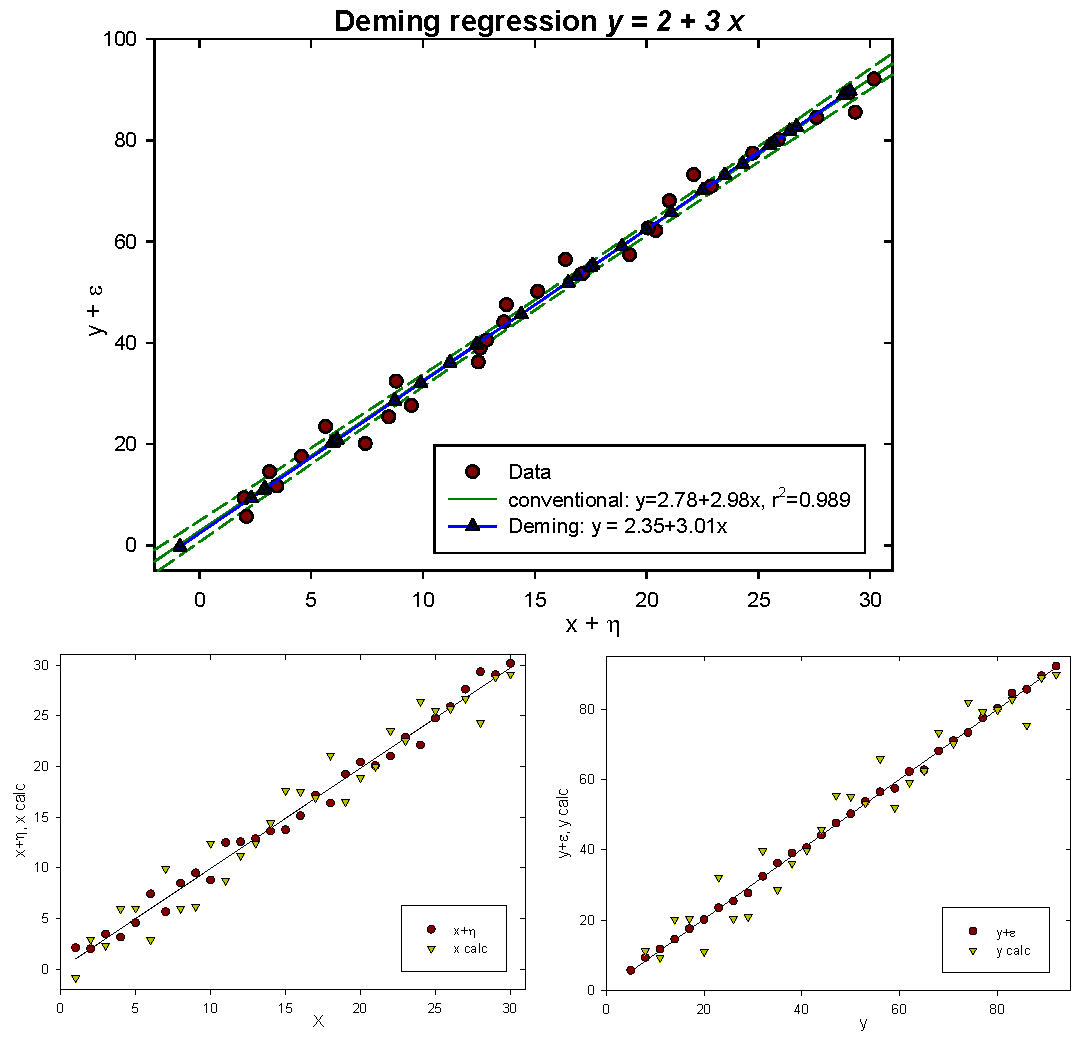
\includegraphics[width=0.75\textwidth]{Graphics/Deming}
\end{figure}

A \Name{Deming}-regression \parencite{Adc-78,Kum-79,Dem-43} is used when both dependent and independent variable have errors (see fig. \ref{fig:Deming}). The errors of dependent and independent variable are assumed independent, normally distributed, and with known ratio of their variance:
\begin{align}
  \AbsVec{y}_i &= \AbsVec{y}_i^* + \epsilon_i \\
  \AbsVec{x}_i &= \AbsVec{x}_i^* + \eta_i \\
  \delta &= \frac{\sigma_\epsilon^2}{\sigma_\eta^2}
\end{align}
The most common problem is that \skalar{\delta} is unknown. In the special case \(\delta = 1 \), \Name{Deming}-regression becomes orthogonal regression, which minimises the sum of squared distances between data points and regression line perpendicular to the line.

As estimate for \( \epsilon \) and \( \eta \) we can use the reciprocals of the reading error (obtained by error propagation, where necessary), divided by \(\sqrt{k} \) if they are the average of \( k \) measurements.

Then the weighted sum of squared distances is minimised
\begin{equation}
  \mathrm{RSS} = \sum_{i=1}^n\left(\frac{\epsilon_i^2}{\sigma^2_\epsilon} + \frac{\eta_i^2}{\sigma^2_\eta}\right)
               = \frac{1}{\sigma^2_\epsilon} \sum_{i=1}^n\left((\AbsVec{y}_i - \beta_0 - \beta_1 \AbsVec{x}_i^*)^2 + \delta (\AbsVec{x}_i - \AbsVec{y}_i^*)^2\right)
\end{equation}
With \(s_\AbsVec{xx} = 1/n \sum_{i=1}^n(\AbsVec{x}_i - \bar{\AbsVec{x}})^2 \) the sample variance of \AbsVec{x}, \(s_\AbsVec{yy} = 1/n \sum_{i=1}^n(\AbsVec{y}_i - \bar{\AbsVec{y}})^2 \) the sample variance of \AbsVec{y}, and \(s_\AbsVec{xy} = 1/n \sum_{i=1}^n\left((\AbsVec{x}_i - \bar{\AbsVec{x}})(\AbsVec{y}_i - \bar{\AbsVec{y}})\right) \)  the sample covariance of \AbsVec{x,y}. Note the small s, which distinguishes these second order moments from the first order ones used above.

We then get
\begin{align}
  b              &= \frac{s_\AbsVec{yy} - \delta s_\AbsVec{xx} + \sqrt{(s_\AbsVec{yy} - \delta s_\AbsVec{xx})^2 + 4 \delta s^2_\AbsVec{xy}}}{2 s_\AbsVec{xy}} \\
  a              &= \bar{\AbsVec{y}} - b \bar{\AbsVec{x}}  \\
  \hat{\AbsVec{x}}_i &= \AbsVec{x}_i + \frac{b}{b^2 + \delta}(\AbsVec{y}_i - a - b\AbsVec{x}_i)\\
\end{align}

The errors of the parameters are not available analytically and must be determined by bootstrapping.

\begin{lstlisting}[caption=Deming-regression]
  PROCEDURE Deming (CONST x, y : VectorTyp; delta : double;
                    VAR xCalc, yCalc : VectorTyp; VAR Res : ResultTyp);

  VAR i, n, s                                : WORD;
      Sx, Sy, sxx, syy, sxy, xMean, yMean,b_ : double;
      Significance                           : SignificanceType;
      c                                      : CHAR;

  BEGIN
    IF VectorLength(x) <> VectorLength(y)
      THEN
        BEGIN
          RegressionError := TRUE;
          c := WriteErrorMessage('Deming regression: unequal length of data vectors');
          EXIT;
        END;
    n := VectorLength(x);
    s := 0;                                                   // calculate means
    Sx := 0;
    Sy := 0;
    FOR i := 1 TO n DO
      BEGIN
        IF IsNaN(GetVectorElement(x, i)) OR IsNaN(GetVectorElement(y, i))
          THEN
          ELSE
            BEGIN
              INC(s);                                        // valid data pairs
              Sx := Sx + GetVectorElement(x, i);
              Sy := Sy + GetVectorElement(y, i);
            END;
      END;
    xMean := Sx / s;                                    // calculate 2nd moments
    yMean := Sy / s;
    sxx := 0;
    syy := 0;
    sxy := 0;
    FOR i := 1 TO n DO
      BEGIN
        IF IsNaN(GetVectorElement(x, i)) OR IsNaN(GetVectorElement(y, i))
          THEN
          ELSE
            BEGIN
              sxx := sxx + Sqr(GetVectorElement(x, i) - xMean);
              syy := syy + Sqr(GetVectorElement(y, i) - yMean);
              sxy := sxy + (GetVectorElement(x, i) - xMean) * (GetVectorElement(y, i) - yMean)
            END;
      END;
     sxx := sxx/s; // sample variance x
     syy := syy/s; // sample variance y
     sxy := sxy/s; // sample covariance x,y                  // calculate params
     Res.b := (syy - delta*sxx + Sqrt((syy-delta*sxx)*(syy-delta*sxx) + 4*delta*sxy*sxy))
               / (2*sxy);
     Res.sb := NaN; // Deming regression doesn't provide error estimates
     Res.a := yMean - Res.b*xMean;
     Res.sa := NaN;
     Res.r := QuadrantCorrelation(x, y, Significance);
     Res.P0 := Significance.P0;
     Res.t := Significance.Testvalue; // actually chi^2, not t
     CreateVector(xCalc, n, 0.0);                    // calculate xCalc and yCalc
     CreateVector(yCalc, n, 0.0);
     b_ := Res.b/(Res.b*Res.b + delta);
     FOR i := 1 TO n DO
       BEGIN
         IF IsNaN(GetVectorElement(x, i)) OR IsNaN(GetVectorElement(y, i))
           THEN
           ELSE
             BEGIN
               SetVectorElement(xCalc, i, GetVectorElement(x, i) + (GetVectorElement(y, i) -
                                Res.a - Res.b * GetVectorElement(x, i)));
               SetVectorElement(yCalc, i, Res.a + Res.b * GetVectorElement(xCalc, i));
             END;
       END;
  END;
\end{lstlisting}

\section{\Name{Theil-Sen-Kendall}-estimator for noisy data}

In this method \parencite{The-50}, the median of the slopes of all \( n(n-1)/2 \) lines connecting two data points ( \( (\AbsVec{y}_j - \AbsVec{y}_i)/(\AbsVec{x}_j - \AbsVec{x}_i)\ \forall\ i,j \in [1\ldots n], i \neq j, \AbsVec{x}_j \neq \AbsVec{x}_i \)) is taken as slope of the regression line \skalar{b}. The last condition is relevant when replicate data are available for the same \AbsVec{x}. Since the determination of slope is the more precise, the larger the difference \(\abs(\AbsVec{x}_j - \AbsVec{x}_i) \) is, one can test for a minimal difference rather than for a difference of zero. The average distance is \(\frac{\max(\AbsVec{x}) - \min(\AbsVec{x})}{n} \), so the significant distance is chosen lower by some arbitrary factor.

The intercept is calculated from \(a = \tilde{\AbsVec{y}} - b \tilde{\AbsVec{x}} \). The alternative estimator for \skalar{a}, the median of the intercept of all the lines, is less robust.

It is possible to weigh the slopes by \(\AbsVec{x}_1 - \AbsVec{x}_2 \) on the grounds that larger distances allow a more accurate determination of slopes.

An estimate for the imprecision of slope and intercept can be calculated from their interquartile distance: \((Q_3 - Q_1) / 2 \). This is similar to the standard deviation in least squares regression, except that it includes the centre \SI{50}{\%} rather than \SI{68}{\%} of values. Similar again to linear regression, estimates of error require sufficient data, \(n > 600 \), to be meaningful.

The \Name{Theil-Sen-Kendall}-estimator has the following properties:
\begin{itemize}
  \item{The \Name{Kendall} \(\tau \) rank correlation coefficient between \(\AbsVec{x}_i \) and the corresponding residual \((\AbsVec{y}_i - \hat{\AbsVec{y}}_i) \) is approximately zero, that is, the probability of a point being above or below the regression line does not depend on \(\AbsVec{x}_i \).}
  \item{The median of the residuals is approximately zero; that is, the fit line passes above and below equal numbers of points. }
  \item{The estimates are more robust against noise than the least squares estimator, \(1 - 1/\sqrt{2} \approx \SI{30}{\%} \) of the data may be arbitrarily corrupted before accuracy drops.}
  \item{The non-parametric \Name{Theil-Sen-Kendall}-estimator is almost as efficient as the parametric least squares method in the absence of outliers and normality violations, and much better is these conditions are not met.}
\end{itemize}

An even more robust method for slope calculation is to calculate first the median of all lines going through an \(\AbsVec{x}_i \), and then calculate the median of those for all \AbsVec{x}  \parencite{Sie-82}. The breakdown point of this method is \SI{50}{\%} corrupted data. However, this method is computationally more expensive, it also requires repeat measurements for each \(\AbsVec{x}_i \).

With the \Name{Theil-Sen-Kendall}-estimator being a non-parametric method of linear regression, it makes sense to also use a non-parametric correlation coefficient, here the quadrant correlation (see subsection \ref{text:quadrant} on page \pageref{text:quadrant}). The significance of \texttt{Res.P0} is calculated from a \(\chi^2 \) test with \(\nu = 1 \), thus \texttt{Res.t} actually contains \(\chi^2 \).

\begin{lstlisting}[caption=Theil-Sen-Kendall-estimator]
  PROCEDURE TheilSenKendall (CONST x, y : VectorTyp; VAR yCalc : VectorTyp;
                             VAR Res : ResultTyp);

  VAR i, j, n, s                                                       : WORD;
      Slopes, Slopes_big, Intercepts, Intercepts_big, xSorted, ySorted : VectorTyp;
      x1, x2, y1, y2, xmin, xmax, xdiff, Sx, Sy, xMed, yMed            : double;
      Significance                                                     : SignificanceType;
      c                                                                : CHAR;
      unknown                                                          : BOOLEAN;

  BEGIN
    IF VectorLength(x) <> VectorLength(y)
      THEN
        BEGIN
          RegressionError := TRUE;
          c := WriteErrorMessage('Linear regression: unequal Length OF dependent AND independent data vector');
          EXIT;
        END;
    n := VectorLength(x);
    s := 0;
    CreateVector(Slopes_big, Round(n*(n-1)/2 + 0.5), 0.0);   // maximal possible number OF slopes
    xmax := FindLargest(x);
    xmin := FindSmallest(x);
    xdiff := (xmax - xmin) / (5 * n);  // factor 5 IS arbitrary
    FOR i := 1 TO n DO
       FOR j := Succ(i) TO n DO
         BEGIN
           x1 := GetVectorElement(x, i);
           x2 := GetVectorElement(x, j);
           y1 := GetVectorElement(y, i);
           y2 := GetVectorElement(y, j);
           unknown :=  IsNaN(x1) OR IsNaN(x2) OR  IsNaN(y1) OR IsNaN(y2);
           IF (Abs(x1 - x2) < xdiff) OR unknown
             THEN
             ELSE
               BEGIN
                 INC(s);
                 SetVectorElement(Slopes_big, s, (y1-y2)/(x1-x2));
               END;
         END;
     CreateVector(slopes, s, 0.0);
     FOR i := 1 TO s DO  // remove any empty values from slope vector
       SetVectorElement(slopes, i, GetVectorElement(slopes_big, i));
     DestroyVector(Slopes_big);
     Res.b := Median(slopes);
     Res.sb := (Quantile(slopes, 0.75) - Quantile(slopes, 0.25)) / 2;
     CopyVector(x, xSorted);
     xMed := Median(xSorted);
     CopyVector(y, ySorted);
     yMed := Median(ySorted);
     Res.a := yMed - Res.b * xMed; // most stable estimator FOR intercept
     CreateVector(Intercepts_big, n, 0.0);
     s := 0;
     FOR i := 1 TO n DO  // calculate intercepts FOR all x/y pairs
       IF IsNan(GetVectorElement(x, i)) OR IsNaN(GetVectorElement(y, i))
         THEN
         ELSE
           BEGIN
             SetVectorElement(Intercepts_big, i, GetVectorElement(y, i) - Res.b * GetVectorElement(x, i));
             INC(s);
           END;
     CreateVector(Intercepts, s, 0.0);
     FOR i := 1 TO s DO  // remove any empty values from intercept vector
       SetVectorElement(Intercepts, i, GetVectorElement(Intercepts_big, i));
     DestroyVector(Intercepts_big);
     Res.sa := (Quantile(intercepts, 0.75) - Quantile(intercepts, 0.25)) / 2;
     Res.r := QuadrantCorrelation(x, y, Significance);
     Res.P0 := Significance.P0;
     Res.t := Significance.Testvalue; // actually chi^2, NOT t
     CreateVector(yCalc, n, 0.0);
     FOR i := 1 TO n DO
       SetVectorElement(yCalc, i, Res.a + Res.b * GetVectorElement(x, i));
     DestroyVector(xSorted);
     DestroyVector(ySorted);
     DestroyVector(Slopes);
     DestroyVector(Intercepts);
  END;
\end{lstlisting}

\section{The direct plot of \Name{Eisenthal \& Cornish-Bowden}}

\begin{sidewaysfigure}
 \caption{The direct plot of \Name{Eisenthal \& Cornish-Bowden} with pseudo-random noise added to a \Name{Henri-Michaelis-Menten}-curve with \(K_\mathrm{M} = 1.0 \) and \(V_\mathrm{max} = 1.0 \). \emph{Left}: Most lines intersect inside the red ellipse. \emph{Centre}: Distribution of estimates for \skalar{K_\mathrm{M}} and \skalar{V_\mathrm{max}} (extreme outliers not shown for clarity). Note how the outliers pull the arithmetic mean (\emph{dotted line}) outside the interquartile boxes. The median (\emph{drawn-out line}) is a much better estimator of position. \emph{Right}: Plot of data, estimated curve and residuals. Note also how even a modest amount of random noise pulls the estimates away from the ``true'' parameters, this effect is stronger for \skalar{K_\mathrm{M}} than for \skalar{V_\mathrm{max}}. }
 \label{fig:Eisenthal}
 \centering
 \subfloat{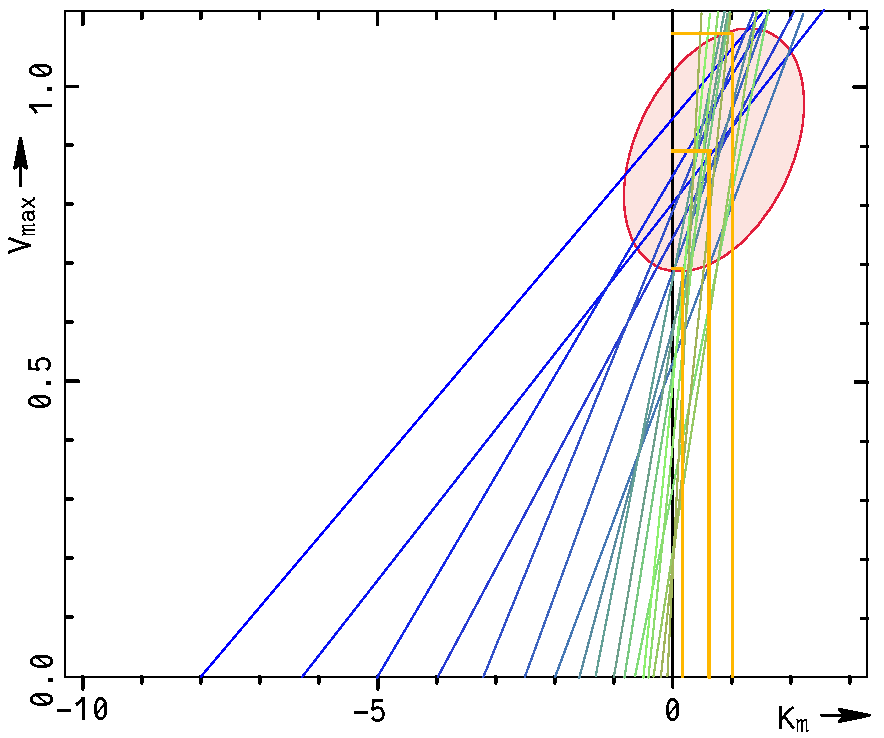
\includegraphics[width=0.3\textwidth]{Graphics/Eisenthal1}}\hfill
 \subfloat{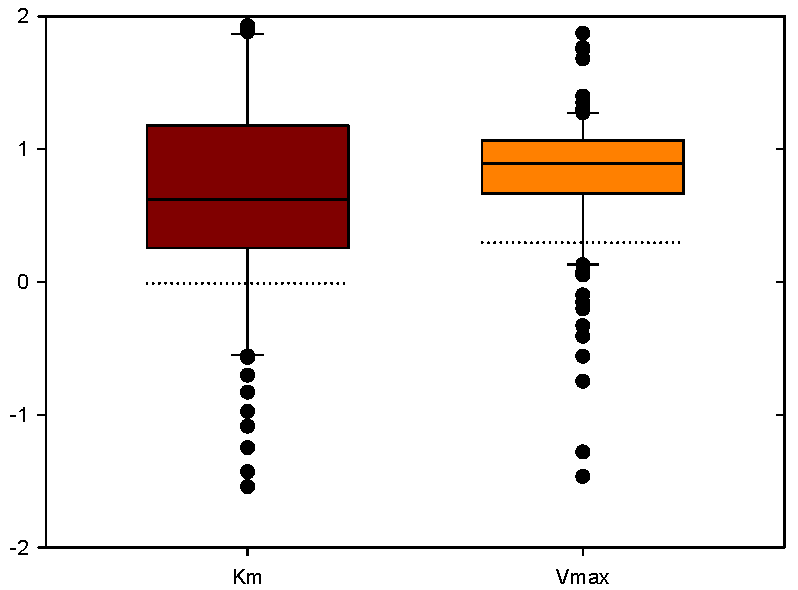
\includegraphics[width=0.3\textwidth]{Graphics/Eisenthal3}}\hfill
 \subfloat{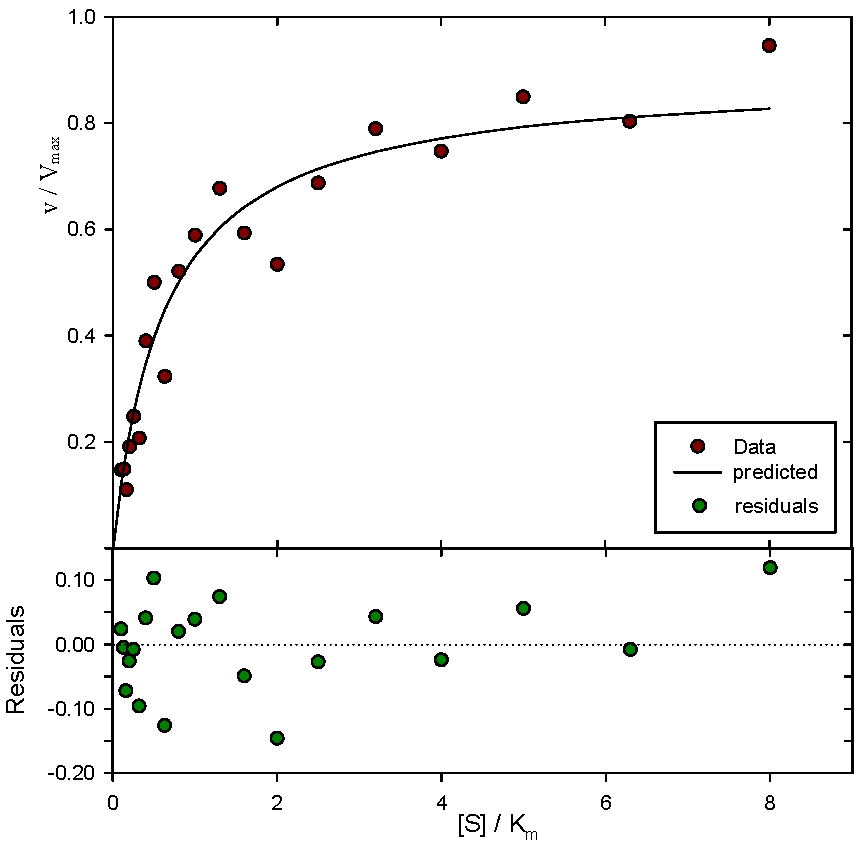
\includegraphics[width=0.3\textwidth]{Graphics/Eisenthal2}}\\
\end{sidewaysfigure}

This method is relevant for enzyme kinetics data, that is the measurement of the reaction velocity \skalar{v} as function of substrate concentration \skalar{[S]}, which is described by the \Name{Henri-Michaelis-Menten}- (HMM-) equation:
\begin{equation}
   v = \frac{V_\mathrm{max} [S]}{K_\mathrm{M} + [S]}
\end{equation}
As mentioned earlier, for such hyperbolic relationships linearising regression may be used, but with significant bias. In particular, estimates of the \Name{Michaelis}-constant \skalar{K_\mathrm{M}} is error-prone.

As \Name{Eisenthal \& Cornish-Bowden} \parencite{Eis-74,Cor-74} realised, if one places lines through the substrate concentrations on the \skalar{x}-axis and the corresponding velocity on the \skalar{y}-axis, all these lines should intersect at \((K_\mathrm{M}, V_\mathrm{max}) \). In practice, one gets a cloud of \(\frac{n (n-1)}{2} \)  intersection points due to experimental noise (see fig. \ref{fig:Eisenthal}). Thus, the median of all intersections between the lines can be used as an unbiased, non-parametric estimator for these two parameters.

The parameters can be calculated from any pair \skalar{i, j} of measured \([S], v \) by
 \begin{align}
   V_{i,j} &= \frac{[S]_i - [S]_j}{\frac{[S]_i}{v_i} - \frac{[S]_j}{v_j}} \\
   K_{i,j} &= \frac{v_j - v_i}{\frac{v_i}{[S]_i} - \frac{v_j}{[S]_j}}
 \end{align}

\begin{lstlisting}[caption=Direct plot]
PROCEDURE Eisenthal (CONST Substrate, Velocity : VectorTyp; VAR yCalc : VectorTyp;
                           VAR Res : ResultTyp);

VAR Km, Vmax, Km_big, Vmax_big : VectorTyp;
    i, j, n, s                 : WORD;
    c                          : CHAR;
    SI, vi, Sj, vj             : double;
    Significance               : SignificanceType;

BEGIN
  IF VectorLength(Substrate) <> VectorLength(Velocity)
    THEN
      BEGIN
        RegressionError := TRUE;
        c := WriteErrorMessage('Direct plot: unequal Length OF dependent AND independent data vector');
        EXIT;
      END;
  n := VectorLength(Substrate);
  s := 0;
  CreateVector(Km_big, Round(n*(n-1)/2 + 0.5), 0.0);   // maximal possible number OF pairs
  CreateVector(Vmax_big, Round(n*(n-1)/2 + 0.5), 0.0);
  FOR i := 1 TO n DO
     FOR j := Succ(i) TO n DO
       BEGIN
         SI := GetVectorElement(Substrate, i);
         Vi := GetVectorElement(Velocity, i);
         Sj := GetVectorElement(Substrate, j);
         Vj := GetVectorElement(Velocity, j);
         IF (IsNaN(SI) OR IsNaN(vi) OR  IsNaN(Sj) OR IsNaN(vj))
           THEN
             // ignore
           ELSE
             BEGIN
               INC(s);
               SetVectorElement(Km_big,   s, (vj - vi) / (vi/SI - vj/Sj));
               SetVectorElement(Vmax_big, s, (SI - Sj) / (SI/vi - Sj/vj));
             END;
       END;
   CreateVector(Km, s, 0.0);
   CreateVector(Vmax, s, 0.0);
   FOR i := 1 TO s DO  // remove any empty values from result vectors
     BEGIN
       SetVectorElement(Km, i, GetVectorElement(Km_big, i));
       SetVectorElement(Vmax, i, GetVectorElement(Vmax_big, i));
     END;
   DestroyVector(Km_big);
   DestroyVector(Vmax_big);
   Res.a := Median(Km);
   Res.sa := (Quantile(Km, 0.75) - Quantile(Km, 0.25)) / 2;
   Res.b := Median(Vmax);
   Res.sb := (Quantile(Vmax, 0.75) - Quantile(Vmax, 0.25)) / 2;
   FOR i := 1 TO s DO
     Writeln(i:3, ' ', GetVectorElement(Km, i):3:3, ' ', GetVectorElement(Vmax, i):3:3);
   Res.r := QuadrantCorrelation(Substrate, Velocity, Significance);
   Res.P0 := Significance.P0;
   Res.t := Significance.Testvalue; // actually chi^2, NOT t
   CreateVector(yCalc, n, 0.0);
   FOR i := 1 TO n DO
     BEGIN
       SI := GetVectorElement(Substrate, i);
       IF IsNaN(SI)
         THEN
           SetVectorElement(yCalc, i, NaN)
         ELSE
           SetVectorElement(yCalc, i, Res.b * SI / (Res.a + SI));
     END;
  DestroyVector(Km);
  DestroyVector(Vmax);
END;

END.
\end{lstlisting}

\section{Aberrant data points}

If the data set \AbsVec{x,y} contains outliers, that is, data points with an error much larger than the other points, the calculated slope will hardly be affected. However, the standard deviations for the parameters will be increased and \skalar{r} decreased. Such outliers should be identified and removed from the data set. On the other hand, data points with high leverage, that is, \skalar{\AbsVec{x}_i} is far away from \skalar{\bar{\AbsVec{x}}}, will strongly affect the parameters.

It is, however, important to use consistent rules for identification of aberrant points. Arbitrary removal of data points which may not fit with ones hypothesis will seriously bias the results and render them useless.

\subsection{Leverage points}

With
\begin{equation}\label{eqn:leverage}
  \arr{H} = \arr{X} (\arr{X}^T \arr{X})^{-1} \arr{X}^T
\end{equation}
the hat-matrix, its \skalar{i}th diagonal element \(\AbsVec{h}_{ii} \) is the \textbf{leverage} of \skalar{\AbsVec{x}_i}. It describes, how much this point will influence the calculated parameters of the regression and is largest for those \skalar{\AbsVec{x}_i} that are furthest away from \skalar{\bar{\AbsVec{x}}_i}. For a simple linear regression,
\begin{equation}
  \AbsVec{h}_{ii} = \frac{1}{n} - \frac{(\AbsVec{x}_i - \bar{\AbsVec{x}})^2}{\sum_{j=1}^n{(\AbsVec{x}_j - \bar{\AbsVec{x}})^2}}
\end{equation}
\( 0 \leq \AbsVec{h}_{ii} \leq 1 \) and any \( \AbsVec{h}_{ii} > \frac{3q}{n} \) is considered high leverage. \skalar{q} is the number of fitted parameters (including intercept).

With those definitions,
\begin{equation}
  \AbsVec{t}_i = \frac{\hat{\epsilon}_i}{\hat{\sigma} \sqrt{1-\AbsVec{h}_{ii}}}
\end{equation}
is called the \textbf{internally \Name{Student}ised residual}. If the absolute value of this residual for any data point exceeds 3, this point can be considered an outlier. If a data point is suspected of being an outlier, it should be excluded from the summation in eqn. \ref{eqn:sigma}, and \skalar{n} in its denominator must be decreased accordingly. However, before it is removed from the data set, make sure that it does not result from an incomplete model!

\subsection{Outliers}

Unlike the errors \(\epsilon_i \) of the measured \AbsVec{y}, the residuals \(\hat{\epsilon}_i = \AbsVec{y}_i - \hat{\AbsVec{y}}_i \) obtained from regression cannot be independent from each other, as their sum must equal zero. Their value decreases with increasing \(\AbsVec{x}_i - \bar{\AbsVec{x}} \). Their variance can be estimated as
\begin{equation}\label{eqn:sigma}
  \hat{\sigma}^2 = \frac{1}{(n-q)} \sum_{i=1}^n{\hat{\epsilon}_i^2} = \frac{1}{(n-q)} \sum_{i=1}^n{(\AbsVec{y}_i - \hat{\AbsVec{y}}_i)^2}
\end{equation}
with \skalar{q} the number of parameters.

\Name{Cook}'s distance is defined as
\begin{equation}
  D_i = \frac{(\hat{\beta} - \hat{\beta}^{\not i})^T (\arr{X}^T\arr{x}) (\hat{\beta} - \hat{\beta}_{\not i})^2}{(1+q) s^2}
      = \frac{\sum_{j=i}^n{(\bar{\AbsVec{y}}_j - \bar{\AbsVec{y}}_j^{\not i})}}{q \mathrm{MSE}}
\end{equation}
where \( \hat{\beta}_{\not i} \) is the calculated least squares slope and \( \bar{\AbsVec{y}}_j^{\not i} \) the calculated \AbsVec{y}  from a refitted regression model in which observation \skalar{i} has been omitted. \acs{MSE} the mean squared error. Values with a \Name{Cook}'s distance of more than four times the mean are suspicious, this measure is somewhat more sensitive than other measures of outliers.

\section{Shrinkage}

Sometimes, the relative importance of the variables in \arr{X} is unknown. In such cases, it is possible to constrain the sum of parameters \(\beta \), and thereby improve their variance \parencite[chapter 6]{Jam-13}.

\subsection{Ridge regression}

In ridge regression, we look for the minimum of
\begin{equation}
  \min\left[\sum_{i=1}^n{(\AbsVec{y}_i - \hat{\AbsVec{y}})^2} + \lambda \sum_{j=1}^p{\beta_j^2} \right]
\end{equation}
, that is, we minimise the sum of both the residual sum of squares and the \(\ell_2 \)-norm of the parameters (except intercept \(\beta_0 \)), \Foreign{i.e.}, the sum of their squares. The relative weight of the later, \textbf{the shrinkage penalty}, is determined by \(\lambda \in [0\ldots\infty] \). If \(\lambda = 0 \) we have a conventional least squares regression. As \(\lambda \) increases, the estimates for \(\beta_j \) are shrunk toward zero. For each \(\lambda \), there is a budget variable \(s \) so that \(\ell_2(\beta) \leq s \). For small \(\lambda \), \(s \) is large and not restrictive, but as \(\lambda \) increases, \(s \) becomes smaller and eventually limiting.

A least square fit has little bias, but may have a lot of variance, that is, a small change in the training data may result in a significant change of the estimated parameters. This variance increases with \(p \), if \(p > n \) regression isn't even possible. As \(\lambda \) increases, the flexibility of the regression decreases, increasing bias and decreasing variance. As the mean squared error \(\mathrm{MSE} = \frac{\sum{(\AbsVec{y}_i - \hat{\AbsVec{y}})^2}}{n} \) is a function of the sum of squared bias and variance, it has an optimal value at a particular \( \lambda \). Hence, the selection of \( \lambda \) is critical and performed by validation (see section \ref{text:validation} on page \pageref{text:validation}).

Before ridge regression, the data should be \AbsVec{z}-standardised so all variables are on the same scale (namely, standard deviations from mean). Otherwise, the final fit would depend on the scale at which the variables have been measured.

\subsection{Lasso regression}\label{text:lasso}

In ridge regression, all parameters are shrunk in the same way, in other words, ridge regression cannot distinguish between important and irrelevant variables. A small change in the equation rectifies this:
\begin{equation}
  \min\left[\sum_{i=1}^n{(\AbsVec{y}_i - \hat{\AbsVec{y}})^2} + \lambda \sum_{j=1}^p{|\beta_j|} \right]
\end{equation}
, in other words, we use the \(\ell_1 \)-, rather than the \(\ell_2 \)-norm of the parameters. This yields \textbf{sparse models}, that is, some parameters may be set to exactly zero. Their number depends on \(\lambda \).

\paragraph{Method selection:} Lasso regression performs slightly poorer than ridge regression when all predictor variables make a seizable contribution to the predicted variable (signal variables); it is superior when there are irrelevant variables (noise variables). A plot of \acs{MSE} \Foreign{vs} \( \lambda \) will show whether shrinkage should be used at all, or whether simple least square regression is sufficient for the problem. Ridge regression can also uncover correlations between variables (\textbf{grouping}). It is possible to combine lasso- and ridge-regression to \textbf{elastic net regression}:
\begin{equation}
  \min\left[\sum_{i=1}^n{(\AbsVec{y}_i - \hat{\AbsVec{y}})^2} + \lambda_1 \ell_1(\beta) + \lambda_2 \ell_2(\beta) \right]
\end{equation}

\printbibliography[heading=subbibliography]
\end{refsection}
